\chapter{Weighted approximation}\label{chap:Weighted}

In this chapter we give a simplified proof of the main lemma of Berman's paper \cite{Berman} containing the currently best approximation algorithm for weighted $k$-set packing with approximation guarantee $\frac{k+1}{2}$. First the necessary terminology is introduced in Section \ref{sec:Terminology}. Then the algorithm is discussed in Section \ref{sec:Algorithm} and Section \ref{sec:ProofBerman} provides a new proof of the main lemma.

\section{Terminology}\label{sec:Terminology}

\paragraph{Claws} Consider the following setting from \cite{Berman} for this chapter. For a graph, define a $k$-claw $C$ as a subgraph isomorphic to $K_{1,k}$, the complete bipartite graph on 1 and $k$ vertices. For convenience, define a 1-claw to be a singleton set $C$ with $T_C = C$. A claw is a $k$-claw for some $k$. Define the single vertex connected to all other vertices of the claw to be the center $Z_C$. The other vertices of the claw (forming an independent set by definition) are called the talons $T_C$ of the claw. A $k$-claw has $k$ talons and one center vertex. Write $C = Z_C \cup T_C$ for a claw $C$ with center vertex $Z_C$ and talons $T_C$.

\paragraph{Approximation guarantee} Let $G = (V,E)$ be a $k$-claw free graph with a weight $w(v)$ for every vertex $v \in V$. The main theorem of \cite{Berman} is a $\frac{k}{2}$-approximation algorithm for maximum independent set in such a graph. This yields a $\frac{k+1}{2}$-approximation algorithm for weighted $k$-set packing because any packing corresponds to an independent set in a $k+1$-claw free graph. The algorithm searches for claws satisfying certain properties and then adds the talons of the claw to the current independent set $A$ and removes the neighbours of the talons in $A$.

\paragraph{Notation} We will use the following notational conventions. Define for a vertex $v \in V$ its open neighbourhood (or just its neighbourhood) $N(v) = \{ w \in V \mid \{v,w\} \in E \}$ and its closed neighbourhood $N[v] = N(v) \cup \{v\}$. For a subset of the vertices $W \subseteq V$ define its closed neighbourhood $N[W] = \bigcup_{w \in W} N[w]$ and write $N(W) = N[W] \setminus W$ for the (open) neighbourhood of $W$.
%
\begin{defn}
For two given subsets of the vertices $U$ and $A$ write $N(U,A) = N(U) \cap A$, i.e. the neighbourhood of $U$ in $A$.
\end{defn}
%
$N(U,A)$ is called the $A$-neighbourhood of $U$ and we refer to the vertices in $N(U,A)$ as the $A$-neighbours of $U$. Write $N(u,A)$ for $N(\{u\},A)$ for some vertex $u$ and some subset of the vertices $A$.
%
\begin{defn}
By $n(u,A)$, denote a vertex $v \in N(u,A)$ with maximum weight.
\end{defn}
%
If this is not uniquely defined, simply choose a random vertex of the different possibilities. %For a given independent set $A$ we denote $n(u) = n(u,A)$ for short, being a vertex in $N(u,A)$ with maximum weight.

For convenience we introduce the notation $w(U) = \sum_{v \in U} w(v)$ for some subset of the vertices $U \subseteq V$. Even shorter, we write the following.
%
\begin{defn}
$w(U,A) = w(N(U,A))$ and $w(u,A) = w(N(u,A))$.
\end{defn}
%
These are the sums of the weights of the $A$-neighbours of a subset of the vertices $U$ respectively one vertex $u$. These notations extend to different weight functions such as $w^2$, in particular note that $w^2(U,A) = \sum_{v \in N(U,A)} w^2(v) \neq \left( w(U,A) \right)^2$. Now define the following function as in \cite{Berman}.
%
\begin{equation*}
charge(u,v) = \left\{
                \begin{array}{ll}
                  w(u) - \frac{1}{2}w(u,A), & \hbox{if $v = n(u,A)$;} \\
                  0, & \hbox{otherwise.}
                \end{array}
              \right.
\end{equation*}

Now define the following.
%
\begin{defn}
Let $A$ be an independent set in a graph $G = (V,E)$. Define a good claw $C = Z_C \cup T_C$ to be a claw satisfying either of the following properties.
%
\begin{enumerate}
  \item $N(T_C,A) = \emptyset$, i.e. adding $T_C$ to $A$ to obtain another independent set does not require the removal of any sets in $A$; or
  \item The center vertex $Z_c$ is in $A$ and $\sum_{u \in T_C} charge(u,v) > \frac{1}{2}w(v)$.
\end{enumerate}
%
A claw $C$ is called a nice claw if it is a minimal set forming a good claw, i.e. if there is no strict subset of $C$ forming a smaller good claw.
\end{defn}

\section{Two algorithms joining forces}\label{sec:Algorithm}

\subsection{The algorithms \textsc{SquareImp} and \textsc{WishfulThinking}}\label{subsec:Algorithms}

In this setting, define the following algorithm:
%
\begin{quote}
\textsc{SquareImp} \\
$A \leftarrow \emptyset$ \\
While there exists a claw $C$ such that $T_C$ improves $w^2(A)$ \\
\verb"  " $A \leftarrow A \cup T_C \setminus N(T_C,A)$
\end{quote}
%
Now define the following algorithm:
%
\begin{quote}
\textsc{WishfulThinking} \\
$A \leftarrow \emptyset$ \\
While there exists a nice claw $C$ \\
\verb"  " $A \leftarrow A \cup T_C \setminus N(T_C,A)$
\end{quote}
%
These two algorithms can now be linked in the following way.
%
\begin{enumerate}
  \item Every nice claw improves $w^2(A)$, so a run of \textsc{WishfulThinking} forms the initial part of a run of \textsc{SquareImp}. See Section \ref{sec:ProofBerman}.
  \item Consequently, \textsc{WishfulThinking} cannot make more iterations than \textsc{SquareImp}.
  \item When \textsc{SquareImp} terminates it yields an independent set $A$ for which no claw improves $w^2(A)$. Hence there is no more nice claw, so \textsc{WishfulThinking} terminates.
  \item If \textsc{WishfulThinking} terminates, its approximation guarantee is $\frac{k}{2}$. See Subsection \ref{subsec:Approx}.
\end{enumerate}
%
The proof of the approximation guarantee is repeated in Subsection \ref{subsec:Approx} to get some insight into the non-intuitive definitions of the charge function and good claws. The main lemma is the fact that every nice claw improves $w^2(A)$, for which we give a simplified proof in Section \ref{sec:ProofBerman}.

%Berman \cite{Berman} shows that under the assumption that \textsc{WishfulThinking} terminates, its approximation guarantee is $\frac{k}{2}$, which we will repeat in the next subsection to get some insight into the non-intuitive definitions of the charge function and good claws. He argues why every nice claw improves $w^2(A)$, which is the main lemma for which we give a simplified proof in Section \ref{sec:ProofBerman}. Consequently, \textsc{WishfulThinking} cannot make more iterations than \textsc{SquareImp}. When \textsc{SquareImp} terminates with some independent set $A$, there is no more claw that improves $w^2(A)$, and hence there is no more nice claw. So \textsc{WishfulThinking} terminates and hence the approximation guarantee has been proved.

\subsection{The approximation guarantee}\label{subsec:Approx}

We repeat the following proof of \cite{Berman}.
%
\begin{lemma}(\cite[Lemma 1]{Berman})\label{lem:Berman1}
Assume that \textsc{WishfulThinking} has terminated and that $A^*$ is an independent set. Then $\displaystyle \frac{w(A^*)}{w(A)} \leq \frac{k}{2}$.
\end{lemma}
%
\begin{proof}
Let $G = (V,E)$ be the graph and let $A$ be the independent set that has been found using \textsc{WishfulThinking}. Let $A^*$ be any independent set in $G$ (in particular it could be the maximum independent set). We will distribute $w(A^*)$ among the vertices of $A$ such that no vertex $v \in A$ receives more than $\frac{k}{2}w(v)$. This immediately implies the claimed result. The distribution consists of two phases.

In the first phase, every vertex $u \in A^*$ sends to each of its $A$-neighbours $v \in N(u,A)$ a portion of its weight equal to $\frac{1}{2}w(v)$. Note that $N(u,A) \neq \emptyset$ because otherwise $\{u\}$ would be a nice 1-claw and these do not exist when \textsc{WishfulThinking} has terminated.

In this first phase, every vertex $u$ sends a portion of its weight equal to $\frac{1}{2}w(u,A)$. By the definition of the $charge$ function, the portion of its weight that is not distributed yet equals $charge(u,n(u,A))$. In the second phase $u$ sends $charge(u,n(u,A))$ to $n(u,A)$.

Now consider some vertex $v \in A$ in the receiving side of this distribution. In the first phase $v$ gets $\frac{1}{2}w(v)$ from all its neighbours in $A^*$. Because $A^*$ is an independent set and the graph is $k$-claw free, $v$ has at most $k-1$ neighbours in $A^*$. Thus $v$ gets at most $(k-1)\frac{1}{2}w(v) = \frac{k}{2}w(v) - \frac{1}{2}w(v)$ in the first phase.

In the second phase, $v$ receives exactly $\sum_{u \in N(v,A^*)} charge(u,v)$. By the definition of a good claw, this can be at most $\frac{1}{2}w(v)$: otherwise the vertices in $A^*$ sending positive $charge$s to $v$ form the talons of a good claw with $v \in A$ at its center.

Hence every vertex $v \in A$ receives at most $\frac{k}{2}w(v) - \frac{1}{2}w(v) + \frac{1}{2}w(v) = \frac{k}{2}w(v)$, and hence the weight of $A^*$ is at most $\frac{k}{2}$ times as much as the weight of $A$.
\end{proof}

As noted, this yields a $\frac{k}{2}$-approximation for the weighted independent set problem in $k$-claw free graphs, which results in a $\frac{k+1}{2}$-approximation for weighted $k$-set packing.

\paragraph{Instructive example} Berman \cite{Berman} proceeds with an example of an instance where an iteration of \textsc{WishfulThinking} in fact decreases $w(A)$, which is the function it is in fact trying to maximise. This is contra-intuitive: we are using a local search technique and from a given solution we might move to a next solution with a worse objective value. However, as we will prove in Section \ref{sec:ProofBerman}, an iteration of \textsc{WishfulThinking} always increases $w^2(A)$ and that suffices for the analysis.

Here is the example, see Figure \ref{fig:Example}. Let $S$ be a subset of the current independent set $A$ depicted at the bottom of Figure \ref{fig:Example} and let $T$ be a subset of the vertices in $V \setminus A$ depicted at the top. Write $S = \{s_1, \ldots, s_5\}$ with $w(s_i) = 10$ for $i=1,\ldots,5$, and $T = \{t_1, t_2\}$ with $w(t_1) = w(t_2) = 18$. Let $n(t_i,A) = s_3$ for $i=1,2$.

%\begin{figure}
%        \centering
%        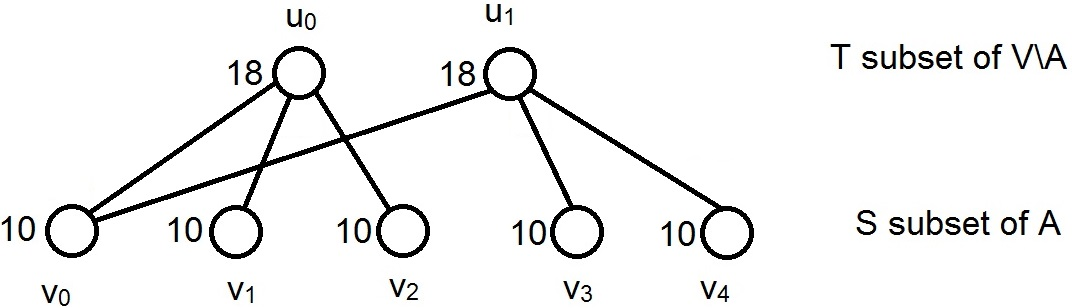
\includegraphics[width = \textwidth]{Images/Example.jpg}
%        \caption{An example where an iteration of \textsc{WishfulThinking} actually decreases $w(A)$. [TODO: Make better picture]}
%        \label{fig:Example}
%\end{figure}

\begin{figure}
\centering
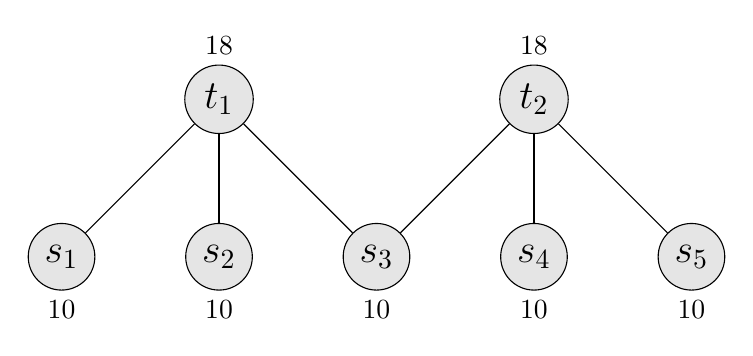
\begin{tikzpicture}[node distance = 2cm, main node/.style={circle,fill=black!10,draw,font=\sffamily\Large\bfseries}]
%[->,>=stealth',shorten >=1pt,auto,node distance=3cm,
  %thick,main node/.style={circle,fill=blue!20,draw,font=\sffamily\Large\bfseries}]
\node[main node, label=below:10] (A) {$s_1$};
\node[main node, label=below:10, right of=A] (B) {$s_2$};
\node[main node, label=below:10, right of=B] (C) {$s_3$};
\node[main node, label=below:10, right of=C] (D) {$s_4$};
\node[main node, label=below:10, right of=D] (E) {$s_5$};
\node[main node, label=above:18, above of=B] (F) {$t_1$};
\node[main node, label=above:18, above of=D] (G) {$t_2$};
\draw (A) -- (F);
\draw (B) -- (F);
\draw (C) -- (F);
\draw (C) -- (G);
\draw (D) -- (G);
\draw (E) -- (G);
\end{tikzpicture}
\caption{An example where an iteration of \textsc{WishfulThinking} actually decreases $w(A)$. The bottom vertices are in $S \subseteq A$ and the top vertices are in $T \subseteq V \setminus A$.}
\label{fig:Example}
\end{figure}

We claim that $\{s_3\} \cup \{t_1, t_2\}$ is a nice claw. To see this, note that $charge(t_i,s_3) = w(t_i) - \frac{1}{2}w(t_i,A) = 18 - \frac{1}{2}(10 + 10 + 10) = 3$. So for $s_3$ we have $\sum_{t_i} charge(t_i,s_3) = 3 + 3 = 6$, which is larger than $\frac{1}{2}w(s_3) = 5$. So all conditions are satisfied and $\{s_3\} \cup \{t_1, t_2\}$ is a good claw, and because it is minimal it is also a nice claw.

However, adding $T$ and removing $N(T,S) = S$ means adding two sets of weight 18 and removing 5 sets of weight 10. Hence $w(A)$ decreases by 14. But the squared weight function increases: the gain is twice $18^2$ and the loss is five times $10^2$, so it increases by $648 - 500 = 148$. In fact, elementary calculus shows that $w^c$ increases in this example for $c > \frac{\log 5 - \log 2}{\log 18 - \log 10} \approx 1.56$, or in a more general setting, for $c > \frac{\log |S| - \log |T|}{\log w(s_i) - \log w(t_i)}$. See also \cite{BermanWeighted2} for results on using the misdirected weight function $w^c$ for some $c \neq 1$.

%\paragraph{Other weight functions than $w$} Intuitively, what is the crucial point why $w^2$ might behave differently than $w$? In general, looking at the squared weight function (or at $w^c$ for any $c>1$) is slightly more biased towards larger weights. When a vertex has weight $m$ and we add 1 to its weight, $w$ increases by 1 while $w^2$ increases by $2m+1$. The square of the weight of one vertex might be more than the weight of two vertices. $w^2$ prefers one vertex of weight 3 to two vertices of weight 2, while $w$ prefers the two vertices of weight 2 to the singly vertex of weight 3. So by guiding the search by $w^2$ rather than $w$, an iteration might decrease the real objective function but it is more difficult to get stuck in an inferior locally optimal solution.

\subsection{A new observation}\label{subsec:Observation}

For the independent set problem in $k$-claw free graphs the use of $w^2$ rather than $w$ can be advantageous due to the following observation. Let $A$ be some independent set and let $u$ be some vertex not in $A$.
%
\begin{equation*}
\sum_{t \in N(u,A)} w^2(t) \leq \sum_{t \in N(u,A)} \left( w(t) \left( \max_{t \in N(u,A)} w(t) \right) \right) = \left( \max_{t \in N(u,A)} w(t) \right) \sum_{t \in N(u,A)} w(t).
\end{equation*}
%
This proofs the following observation.
%
\begin{obs}\label{obs}
$w^2(u,A) \leq n(u,A) w(u,A)$.
\end{obs}

So the squared weight function of a set of vertices is capable of capturing information not only about the sum of the weights but also about the maximum weight. Using this simple observation Berman's proof can be simplified in the next section.

\section{Simplified proof}\label{sec:ProofBerman}

Here is a simplified proof of the main lemma from \cite{Berman} proving that adding a nice claw to the current independent set $A$ improves $w^2(A)$. We believe this proof gives some more insight into what is really happening behind the math thanks to Observation \ref{obs}.
%
\begin{lemma}\label{lem:Berman2}
If $C$ is a nice claw, then $T_C$ improves $w^2(A)$.
\end{lemma}
%
\begin{proof}
Let $A$ be the current independent set and let $C = Z_C \cup T_C = \{v\} \cup T$ be a nice claw. We need to show that the weight of what is added ($T$) is more than the weight of what is lost ($N(T,A)$), so we need to show that
%
\begin{equation}\label{first}
w^2(T) > w^2(T,A),
\end{equation}
%
or equivalently,
%
\begin{equation}\label{second}
w^2(T) - w^2(T,A-\{v\}) > w^2(v).
\end{equation}
%
To proof that for a nice claw \eqref{second} holds, we proof the following claim.
%
\begin{claim}\label{claim1}
Let $C = \{v\} \cup T$ be a nice claw. Then
%
\begin{equation*}
w^2(T,A-\{v\}) \leq \sum_{u \in T} \left( w^2(u,A) - w^2(v) \right).
\end{equation*}
\end{claim}
%
\begin{proof}
%By definition, $w^2(N(T,A))$ is the sum of the squared weights of all neighbours of the talons $T$ in $A$. When we sum over all vertices $u \in T$ and look at $\sum_{u \in T} w^2(N(u,A))$, we count every vertex that is adjacent to $p$ vertices in $T$ exactly $p$ times. In particular, we count $w^2(v)$ exactly $|T|$ times, while on the left-hand side we count it only once. If we thus do not add $w^2(v)$ for every $u \in T$ (by subtracting it again) and add it once at the end, we count $w^2(v)$ exactly once like on the left-hand side. As we may count the squared weights of other vertices multiple times, the right-hand side might sum more positive terms and thus be larger.
By definition, $w^2(T,A-\{v\})$ %equals $\displaystyle \sum_{u \in N(T,A-\{v\})} w^2(u)$.
is the sum of the squared weights of all neighbours of the talons $T$ in $A$ excluding $v$.
Summing over $T$ rather than the neighbourhood of $T$, this can be bounded by $\displaystyle \sum_{u \in T} w^2(u,A-\{v\})$. This is an upper bound, because in this expression vertices that are neighbours of more than one vertex in $T$ are counted multiple times. Therefore, $\displaystyle w^2(T,A-\{v\}) \leq \sum_{u \in T} w^2(u,A-\{v\})$. Noting that $w^2(u,A-\{v\})$ equals $w^2(u,A) - w^2(v)$, the claim follows.
\end{proof}
%
For the first term in \eqref{second}, write $w^2(T) = \sum_{u \in T} w^2(u)$. Now by Claim \ref{claim1}, the following implies \eqref{second}.
%
\begin{equation}\label{fourth}
\sum_{u \in T} \left( w^2(u) - w^2(u,A) + w^2(v) \right) > w^2(v).
\end{equation}
%
To show that \eqref{fourth} holds when $C$ is a nice claw, we proceed to the second claim.
%
\begin{claim}\label{claim2}
Let $C = \{v\} \cup T$ be a nice claw. Then $v = n(u,A)$ for all $u$ in $T$ and
%
\begin{equation}\label{fifth}
w(v) < 2 \sum_{u \in T} charge(u,v).
\end{equation}
\end{claim}
%
\begin{proof}
Equation \eqref{fifth} just follows from the definition stating $\sum_{u \in T} charge(u,v) > \frac{1}{2}w(v)$. Also, as $C$ is a nice claw, it is minimal, implying that every term on the right-hand side of \eqref{fifth} is positive. By the definition of $charge$, this is true only if $v$ is the maximum weight neighbour of $u$ within $A$.
\end{proof}

So proving that \eqref{fourth} holds when $C$ is a nice claw has now been reduced by Claim \ref{claim2} to showing that whenever $charge(u,v)>0$ we have
%
\begin{equation*}
w^2(u) - w^2(u,A) + w^2(v) \geq 2w(v)charge(u,v).
\end{equation*}
%
Here we plugged in \eqref{fifth} only once in the right-hand side. By the definition of $charge$, this boils down to proving that
%
\begin{equation}\label{seventh}
w^2(u) - w^2(u,A) + w^2(v) \geq 2w(u)w(v) - w(v)w(u,A)
\end{equation}
%
holds whenever $v$ is the maximum weight neighbour of $u$.

From this point on we will deviate from the proof of Berman \cite{Berman}. He now scales the quantities, makes a case distinction and rewrites the equations algebraically until it is clear they are indeed true. However, \eqref{seventh} can be shown more easily using Observation \ref{obs}. Plugging this into \eqref{seventh} yields
%
\begin{equation*}
w^2(u) - w(v)w(u,A) + w^2(v) \geq 2w(u)w(v) - w(v)w(u,A).
\end{equation*}
%
The terms $w(v)w(u,A)$ now cancel and what is left is
%
\begin{equation}\label{eighth}
w^2(u) + w^2(v) \geq 2w(u)w(v),
\end{equation}
%
which is obviously true as this is equivalent to
%
\begin{equation*}
(w(u)-w(v))^2 \geq 0.
\end{equation*}
%
We have now proved that when $C$ is a nice claw, \eqref{first} holds, and thus $T_C$ improves $w^2(A)$.
\end{proof}

%\section*{Improving the approximation guarantee}
%
%The above analysis also shows that we cannot simply improve the approximation guarantee to $\frac{d}{c}$ for some $c > 2$. Let us replace the $\frac{1}{2}$ in the definition of $charge(u,v)$ to $\frac{1}{c}$ and the $\frac{1}{2}$ in the definition of a nice (good) claw to $\frac{1}{c}$.
%
%Lemma 1 in Berman can now be easily adapted to hold for any $c>2$. The proof remains exactly the same and \textsc{WishfulThinking} now has an approximation guarantee of $\frac{d}{c}$.
%
%However, Lemma 2 (as above) fails now. The analysis remains exactly the same except for the fact that in \eqref{eighth}, the factor 2 in the right-hand side changes into a $c$. However, with the current analysis, \eqref{eighth} holds only nontrivially for $c=2$. Hence, $w^2$ improves only when $c=2$.
%
%Trying to improve $w^p$ for some $2 < p \in \mathbb{N}$ (also using $c$ rather than 2) yields the same analysis, where \eqref{eighth} translates to
%%
%\begin{equation*}
%w^p(u) + w^p(v) \geq c w(u) w^{p-1}(v).
%\end{equation*}
%%
%This is trivially true for $p = c = 2$. Using the binomial theorem on $(w(u)+w(v))^p$ cancels the term on the right-hand side by letting $c={p \choose 1}=p$, but yields some other terms that seem to hurt.
%
%Note that this is also true for $p = c = 1$, which gives the standard $d$-approximation back. 